\chapter{Method}\label{chapter:first_real_chapter}

\section{Model}
Our method is based on a VAE\cite{kingma2014autoencodingvariationalbayes}. 
% It consist of 3 main parts. The image encoder $p_\theta(x|z)$, the image decoder $q_\phi(z|x)$ and the label decoder $q_\xi(z|x)$. Schematically the model can be seen in Figure \ref{fig:seg-vae-schematic} The image encoder and decoder together are a classical VAE, and will be optimized as such during the pretraining phase.
Similar to Kingma et al., we assume that the data is generated by a random process, which is dependent on the random variable \boldmath{z}. Where \boldmath{z} can be sampled from a prior distribution $p_\theta(z)$. \boldmath{x} is then generated from the conditional distribution $p_\theta(x|z)$. This results in the generative process in Eq.~\ref{eq:vae-process}. Furthermore it is assumed that the true posterior density $p_\theta(z|x) = \frac{p_\theta(x|z)p_\theta(z)}{p_\theta(x)}$ is intractable.  Kingma et al. introduce an approximation of $p_\theta(x|z)$, $q_\phi(z|x)$, also reffered to as the probabilistic encoder.
We extend this with the assumption that there exist an unique mapping $f: X \mapsto Y$, resulting in Eq.~\ref{eq:equalities}. 
\begin{subequations}
    \begin{align}
        p_\theta(x, z) & = p_\theta(x|z)p_\theta(z) \label{eq:vae-process}        \\
        p_\theta(y|z)  & = p_\theta(f(x)|z) = p_\theta(x|z) \label{eq:equalities} \\
        p_\theta(y, z) & = p_\theta(x|z)p_\theta(z)\label{eq:label-process}
    \end{align}
\end{subequations}
Taking Eq.~\ref{eq:equalities}, we can plug that into the Eq.~\ref{eq:beta-elbo}, resulting in Eq.~\ref{eq:beta-label-elbo}.
\begin{equation}
    \label{eq:beta-label-elbo}
    \mathcal{L}_{\beta-label} = \mathbb{E}_{q_{\phi}(z|x)}[\log p(y|z)] - \beta (D_{KL}(q_{\phi}(z|x) || p(z)))
\end{equation}


This results in the following three distributions we want to estimate using an neural network.
\begin{itemize}
    \item $q_\phi(z|x)$ (i.e. image encoder)
    \item $p_\theta(x|z)$ (i.e. image decoder)
    \item $p_\theta(y|z)$ (i.e. label decoder)
\end{itemize}

\subsection{Image Encoder}
The image encoder approximates the latent distribution, $p(z)$. To ensure we can train the encoder using gradient descent, we need to make sure it is fully differentiable. Thus we make use of the reparameterization trick. Using a deterministic mapping $g_\phi(\epsilon, z')$, where $\epsilon$ is an independent random variable and $g_\phi(x)$ is our (deterministic) neural network. Kingma et al. show that using this reparameterization trick, a wide range of distributions can be learned. In our case we use a Gaussian latent space. The reparameterization then becomse $z = \mu + \sigma \epsilon$, where $\mu$ and $\sigma$ are the output of our image encoder network.

\subsection{Image Decoder}
The image decoder approximates the conditional Gaussian distribution $p_\theta(x|z)$. It is used during the pretraining step to prime the image encoder with 'good' initial weights, using the traditional ($\beta$)-VAE training. The hypothesis is, that given that $x$ can be reconstructed from the learned $q_\phi(z|x)$, the learned latent space contains useful features to approximate $p_\theta(y|z)$. In Eq.~\ref{eq:beta-elbo} $log p(x|z)$ can be calculated using Eq.~\ref{eq:log_p_x_z} using a parameterized neural network.

\begin{equation}
    \begin{split}
        log p(x|z)              & = log \mathcal{N}(x; \mu, \sigma^2I) \label{eq:log_p_x_z} \\
        \text{where}~\mu,\sigma & =NN_\phi(z)
    \end{split}
\end{equation}

\subsection{Label Decoder}
The label decoder is similar to the image decoder, except that it approximates a multivariate Bernoulli distribution, instead of an Gaussian. Thus the only difference is the calculation of $log p(y|z)$, which is shown in Eq.~\ref{eq:log_p_y_z}.

\begin{subequations}
    \begin{align}
        log p(y|z)     & = \sum_{i=0}^n y_i log h_i + (1 - y_i)log(1-h_i) \label{eq:log_p_y_z} \\
        \text{where}~h & = softmax(NN_\phi(z))
    \end{align}
\end{subequations}

To improve the sharpness of the labels, additional latent variables are added from higher up the encoder, similar to HVAE. This results in the final loss Eq.~\ref{eq:beta-hvae-label-elbo}.

\begin{equation}
    \label{eq:beta-hvae-label-elbo}
    \mathcal{L}_{\beta-label} = \mathbb{E}_{q_{\phi}(z|x)}[\log p(y|z)] - \beta \sum_{i=0}^n(D_{KL}(q_{\phi}(z_i|x) || p(z_i)))
\end{equation}

\begin{figure}[h]
    \begin{minipage}{0.9\textwidth}
        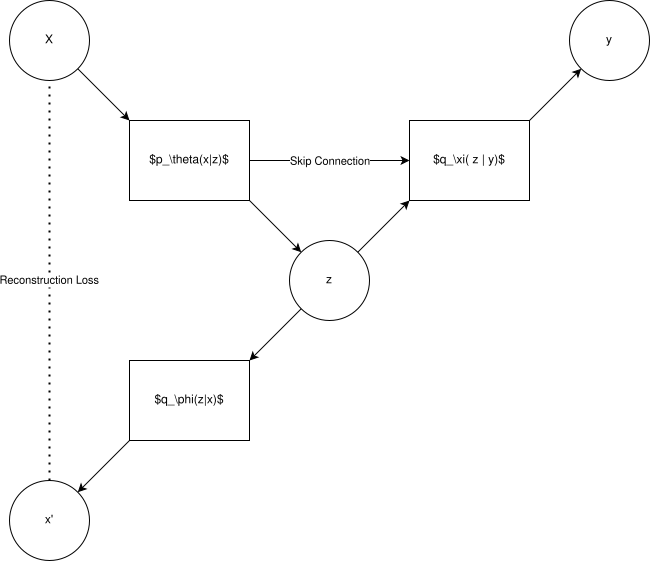
\includegraphics[width=1\textwidth]{figures/model_data_flow.png}
        \caption{The data flow of the various submodels. NOTE: I still want to make this prettier, making it more similar to \ref{fig:hvae-example}}
        \label{fig:seg-vae-schematic}
    \end{minipage}
\end{figure}

\begin{figure}
    \begin{minipage}{0.9\textwidth}
        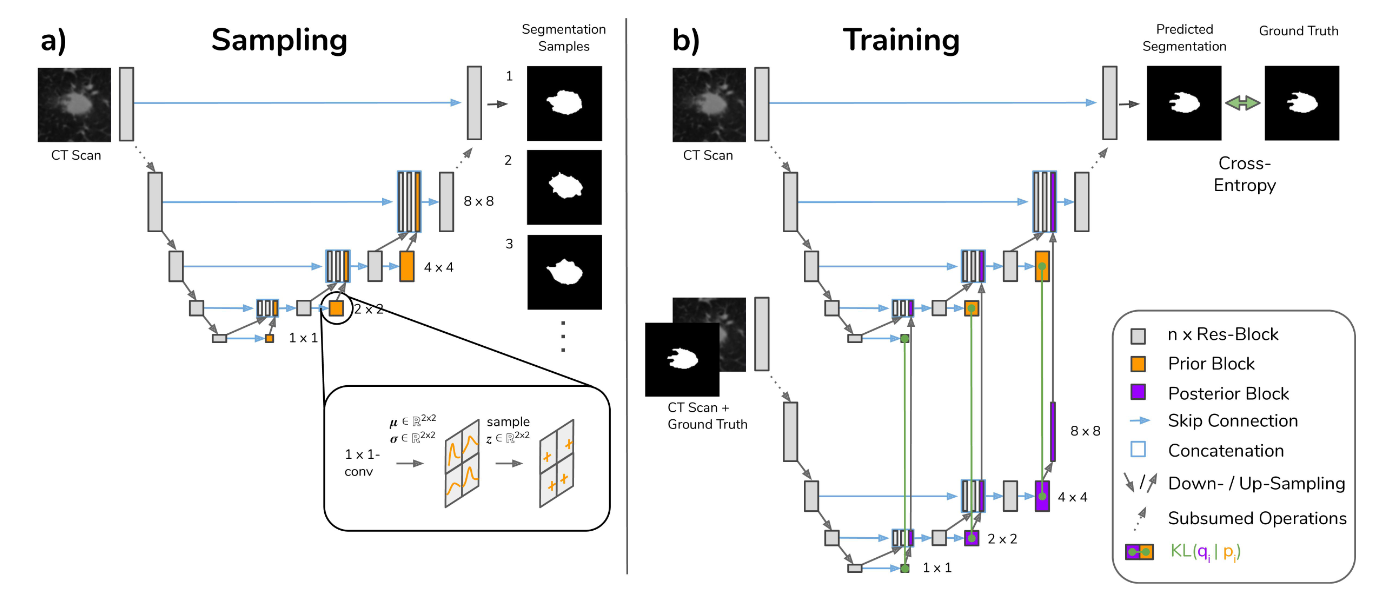
\includegraphics[width=1\textwidth]{figures/h_vae_structure.png}
        \caption{Example of the H-VAE structure. From \cite{kohl2018probabilistic}.}
        \label{fig:hvae-example}
    \end{minipage}
\end{figure}

\section{Training procedure}
\subsection{Pretraining}
First the model is trained as a VAE, in which the unlabeled (full) dataset is used. Various backbones will be tried, however these will be part of the "ablation" study. Currently three backbones are on my radar:
\begin{itemize}
    \item Resnet50 \cite{he2015deep}
    \item VGG16 \cite{simonyan2015deep}
    \item Vision Transformer \cite{dosovitskiy2021image}
\end{itemize}
The dataset used during pretraining can be indepently chosen compared to the finetuning stage. It can either be the same dataset as the finetuning stage, or a more generic, and thus bigger, dataset. 

\subsection{Fine-Tuning}
The second stage will replace the last layer with a new convolutional layer, as it structure changes. The rest of the model will remain structurly the same. The following choices need to be made, and will be done so after experimentation:
\begin{itemize}
    \item How many of the layers do we copy from the VAE?
    \item How many of the layers do we freeze?
\end{itemize}

% \subsection*{Why VAE?}
% By using a VAE bootstrapping can be applied during inference to provide an insight in the certainty of the model, as has been shown by \cite{kohl2018probabilistic}. This certainty estimation from the bootstrapping is crucial in mobile robotics and can be done quickly using batched inference.

\subsection{Loss functions}
Standard loss function for the H-VAE

\begin{equation}
    \lambda_{HVAE}(x) := \EX_{q(z|x)}[log(p(x|z))] - KL(q(z_1|x)||p(z_1)) - \sum_{l=2}^{L} \EX_{q(z_{<l}|x)}[q(z_l| x, z_{<l}) ||p(z_l|z_{<l})]
\end{equation}


Loss function for the Hierarchical Variational Segmenter
\begin{equation}
    f_{\theta, \xi}(x) = p_\theta()
\end{equation}
\begin{equation}
    \lambda_{HVS}(x, y) := CELoss(f_{\theta, \xi}(x), y) - KL(q(z_1|x)||p(z_1)) - \sum_{l=2}^{L} \EX_{q(z_{<l}|x)}[q(z_l| x, z_{<l}) ||p(z_l|z_{<l})]
\end{equation}

\section{Evaluation}

\subsection{Inference}
Due to the variational architecture of the model, the inference can be done either deterministic, by taking the mean of each latent vector. Or variational, by sampling each latent vector. The benefit of sampling is that there is a possibility to use bootstrapping to get an estimate of the uncertainty. Kohl et al. \cite{kohl2018probabilistic} have shown that bootstrapping can be used to produce an uncertainty measure in neural networks. Furthermore, bootstrapping allows for an ensemble which might improve the top-1 accuracy of the model.


\subsection{Metrics}
Within classification the most well-known and widely used metrics are precision (\ref{eq:precision}), recall (\ref{eq:recall}), and F1-score (\ref{eq:f1})\cite{rijsbergen1979information}. Of which the latter is a combination of precision and recall. Within the field of image segmentation, the F1-score is also Sometimes refered to as the Recognition Quality (RQ)
\begin{equation}
    \label{eq:precision}
    \text{Precision} = \frac{TP}{TP + FP}
\end{equation}
\begin{equation}
    \label{eq:recall}
    \text{Recall} = \frac{TP}{TP + FN}
\end{equation}
\begin{equation}
    \label{eq:f1}
    F1 = \text{RQ} = 2 \cdot \frac{\text{Precision} \cdot \text{Recall}}{\text{Precision} + \text{Recall}}
\end{equation}
The Jaccard Index (\ref{eq:jaccard}) is also widely used as it provides a 

\begin{equation}
    \label{eq:jaccard}
    \text{Jaccard Index} = \frac{TP}{TP + FN + FP}
\end{equation}


To determine the quality of the uncertainty estimation produced by bootstrapping, the Expected Callibration Error (ECE), proposed by Naeini et al. \cite{naeini2015obtaining}, will be measured. 

\begin{equation}
    \text{ECE} = \sum_{m=1}^M \frac{|B_m|}{n} \left| \text{acc}(B_m) - \text{conf}(B_m) \right|
\end{equation}
where:
\begin{itemize}
    \item \(M\) is the number of bins.
    \item \(B_m\) is the set of indices of samples whose predicted probabilities fall into the \(m\)-th bin.
    \item \(|B_m|\) is the number of samples in bin \(m\).
    \item \(n\) is the total number of samples.
    \item \(\text{acc}(B_m)\) is the accuracy of the \(m\)-th bin.
    \item \(\text{conf}(B_m)\) is the average confidence of the \(m\)-th bin.
\end{itemize}
